% This is samplepaper.tex, a sample chapter demonstrating the
% LLNCS macro package for Springer Computer Science proceedings;
% Version 2.20 of 2017/10/04
%
\documentclass[runningheads]{llncs}
%
\usepackage{graphicx}
\usepackage{hyperref}
% Used for displaying a sample figure. If possible, figure files should
% be included in EPS format.
%
% If you use the hyperref package, please uncomment the following line
% to display URLs in blue roman font according to Springer's eBook style:
% \renewcommand\UrlFont{\color{blue}\rmfamily}

\begin{document}
%
\title{Voting on Blockchain}
%
%\titlerunning{Abbreviated paper title}
% If the paper title is too long for the running head, you can set
% an abbreviated paper title here
%
\author{Stanisław Barański, Julian Szymanski, Andrzej Sobecki, ktoś z alicante}

% First names are abbreviated in the running head.
% If there are more than two authors, 'et al.' is used.
%
\institute{Faculty of Electronics, Telecommunications and Informatics\\
Gdansk University of Technology\\
Gdansk, Poland\\
\email{s160518@student.pg.edu.gda.pl}}
%
\maketitle              % typeset the header of the contribution
%
\begin{abstract}
In this paper, we propose e-voting system which satisfy transparency, audibility, verifiability and privacy. System is backed by open stellar blockchain.

%JS wypunktować co jest wkładem artykułu

\keywords{Blockchain \and Voting  \and Tokenization} %JS  e? i? Voting 
\end{abstract}


\section{Introduction}


% merge with introduction
\section{State of the art}

\paragraph{Breaking the Encryption Scheme of the Moscow Internet ~\cite{gaudry2019breaking} }

\paragraph{E-voting with blockchain: An e-voting protocol with decentralisation and voter privacy ~\cite{hardwick2018voting} }
Based purely on bitcoin network. Token based on Colored Coins. Can be ripped by sending AS malicious transaction. Very costly. Satisfy almost all properties. Yes, based on trusted party. Like me

\paragraph{An E-voting Protocol Based on Blockchain. ~\cite{liu2017voting}}
Argues to not require TTP, instead introduce inspectors, and if they are corrupted (what we have to assume for pessimistic scenario), the election is also corrupted. But requires pre-registration with bitcoin public key. Or they don't argue any solution or In my opinion it's unpractical.

\paragraph{Blockchain for democratic voting: how blockchain could cast of voter fraud ~\cite{casado2018blockchain} }

\paragraph{Blockchain-enabled e-voting ~\cite{kshetri2018blockchain} }

\paragraph{The future of democracy: Blockchain voting ~\cite{osgood2016future}}

\paragraph{Secret Voting ~\cite{tam_2018} }

\subsection{E-Voting system requirements}
Requirements that robust e-voting system should satisfy follows:
\begin{itemize}
\item \textbf{Immutability}: No one can change their mind after vote is made.
\item \textbf{Verifiability}: Everyone should be able to verify if his vote has been counted correctly.
\item \textbf{Trustless}: Each user should be able to compute results on it's own.
\item \textbf{Scalability}: System should be able to handle large number of votes per second.
\item \textbf{Authorization}: Only authorized voters can vote.
\item \textbf{Un-reusability}: No one can vote more than once.
\item \textbf{Privacy}: Relation between voter and his vote, must be keep in secret. Each voter must be sure about his opinion privacy. 
\item \textbf{Coercion resistance}: It should be illegal to exchange votes.
\item \textbf{Fairness}: No partial results are available until end of election.
\end{itemize}

In this article we propose system that satisfy all of those requirements, based on stellar open blockchain network.

%JS czy to wszystko czy jesli zostanie spelnione to mozna wdrazac w panstwe,
%w dyskusji trzeba sie do tego odniesc 


\section{Verifability, Trustless and Immutability}
 Blockchain technology provides two major properties that are highly desirable in applications like election voting. Those properties are immutability which ensures that no one can modify the data once wrote into a blockchain. Another property is transparency that allows everyone to validates the election correctness and calculate results on its own. In consequences, one can distrust authorities, while trust voting results. 

Blockchain initially introduced by Satoshi Nakamoto in Bitcoin Whitepaper offered one simple application, i.e. ledger for transferring Bitcoin cryptocurrency. 5 years later Vitalik Buterin proposed generalization to this concept by allowing to process not only transactions but also so-called smart contracts which are in fact scripts run on Ethereum platform. Those “scripts” are executed and validated by all Ethereum nodes and use blockchain as persistent storage. This innovation allowed to create domain-specific behavior on top of Ethereum blockchain, leveraging already existing infrastructure.

%\subsection{Tokenization}
Currently, the most popular application of smart contracts is token issuance. Those tokens can represent any arbitrary asset either in the virtual or physical world. One can create tokens for funding his startup; hence token represent company shares. This pattern is called ICO (Initial Coin Offering) or STO (Security Token Offering), alluding to IPO (Initial Public Offering). Another one can issue tokens backed by a physical asset like national currency; bypassing slow and expensive international transfers and taxes from exchanging cryptocurrencies with national currencies. This pattern is called Stable Coin. There are many other token applications particularly vote tokenization, used here in this survey.


\section{System proposition}
The goal of the system is to provide the highest level of transparency while keeping sensitive data private. Additionally, it should be illegal to issue more than one vote token to one elector. Hence there should be a way of identifying and authorizing voters. I decided to use a government authorized polish system
“Profil Zaufany” as an identity provider, with the assumption that every eligible voter is registered there. The total number of votes tokens should be limited to the total number of eligible voters. We assume that this number is publicly available on the day of the election. In consequence, everyone can verify that there were no more token issued. 

\subsection{Stellar platform}
Ethereum provides high flexibility, mainly because of its fully-fledged smart contracts ecosystem, particularly it’s Turing-complete Solidity language. Stellar on the other hand is a blockchain platform specializing just in one application that is asset tokenization. Thus becoming easier, cheaper and faster than general-purpose Ethereum smart contracts. Here We will try to fit election system into Stellar functionality boundaries.


\subsection{Architecture}
\begin{figure}
\begin{verbatim}
                         +                    +
        Government       |      Electoral     |      Blockchain
                         |                    |
                         |                    |
   +-------------------+ |                    |
   | Identity Provider | |                    |
   | (Profil Zaufany)  | |                    |
   +-----------------^-+ |                    |
                     |   |  +---------------+ | +-------------+   +---------+
                     +------> Client Webapp +---> Stellar     +---> Stellar |
                     |   |  +---------------+ | | Horizon API |   | Network |
+--------------------v-+ |                    | +-------------+   +---------+
|Issuance/Authorization| |                    |
|       Server         | |                    |
+----------------------+ |                    |
                         |                    |
                         |                    |
                         |                    |
                         |                    |
                         +                    +

\end{verbatim}
\caption{System architecture}
\label{fig:ascii-box}
\end{figure} 

Proposed system consists of three parties: Government, Electoral and Blockchain. Both Government and Electoral distrust each other, because each of the parties has interest in manipulating the process of election. Electoral demand from Government to be as transparent as possible. Government perform authentication and authorization process to prevent unauthorized votes or double \textit{vote token} issuance.

Ideally \textit{Identity Provider} and \textit{Issuance/Authorization Server} should be separate entities, but we notice pessimistic scenario, where they both cooperate together to manipulate election results.

Ideally, the system should consist only of a client webpage that allows users to interact with the Stellar network, getting rid of the centralized \textit{identity provider} and \textit{issuance/authorization server}. Unfortunately proposed system requires a central authorization server for vote token issuance, thus becoming a single point
of failure. This flaw has been addressed at the end of this paper. There are also many proposals on how to achieve authentication on the blockchain ecosystem, but we won't cover them in this paper.

\subsection{Scalability}

Blockchain is famous for being very slow. Ethereum creator Vitalik Buterin claims that Blockchains face trillema ~\cite{ethereum} which allows them to choose only two of three properties: Decentralization, Security and Scalability. And here is the place where variety of different Blockchain platforms comes out offering something unique. While most conservative Blockchain like Bitcoin and Ethereum put on Security and Decentralization, others offers higher Scalability on the cost of Decentralization and Security. Stellar is one of such solutions. 
At the date of writing, Ethereum is able to process 15 transactions per second (TPS). Whereas Stellar is able to process 1000 operations per seconds (OPS). 

\section{Authentication and Authorization}
Voter obtain authentication token from \textit{identity provider} using one of available methods like OAuth2/OpenID Connect. This token is then presented to \textit{authorization/issuance server}, who can authenticate the request by asking \textit{identity provider}. Next, authorization/issuance server checks in it's local database, if such user have not already issued vote token. Preventing from double \textit{vote token} issuance.

\subsection{Vote Token}
We assume that the number of eligible voters is public information. Hence becoming the value of a maximum number of tokens in this election. After asset creation, issuing accounts have to lockout from creating a new asset, so all participants can be sure that no more tokens are ever created. Additionally, it should be impossible to perform vote, after the end of the election. Unfortunately Stellar doesn’t have such feature build-in, although it can be done by blocking all new token issuance on issuance/authorization server.
Assets in stellar blockchain, are divisible to 7 decimal points. This is an unwanted feature since we don’t want to allow users to vote by just one-tenth of their vote. To prevent it, we will treat 1 vote token as the smallest indivisible amount possible in XDR which is 1 scaled down by a factor of 10,000,000 (this format allows to represent decimal numbers in 7 digit precision, without introduction floating-point arithmetics and it’s innate errors).
Vote option is expressed in strictly encoded 32 byte MEMO field available in blockchain transaction. Frame structure is presented in Fig. \ref{fig:ballot-encoding}. 
\begin{figure}
\begin{verbatim}
+------+-------------------------+-----------------------+---------------+
| Name |     Question code       |     Option code       | Random string |
+------------------------------------------------------------------------+
|      |                         |                       |               |
| Bits | n=ceil(lg(|Questions|)) | m=ceil(lg(|Options|)) |  r=256+n+m    |
|      |                         |                       |               |
+------+-------------------------+-----------------------+---------------+

\end{verbatim}
\caption{Voting ballot encoded in 32 byte MEMO field}
\label{fig:ballot-encoding}
\end{figure} 

We propose questions and options for multi option ballots, and further extensions. Random string of bits is added to prevent from preliminary results that could be achieved by calculating the same MEMO fields.
The MEMO field is encrypted using publicly available special public key, preventing from preliminary results. At the end of election the issuer publish corresponding private key, allowing everyone to calculate the election results on their own. Random string of bits is added to prevent from preliminary results that could be achieved by summing equal memo fields.

\section{Privacy}
\label{privacy}
Privacy seems to be the hardest problem to achieve. Especially in conjunction with authorization and data stored public blockchain. There are some propositions on how to solve this problem. 

First one is to allow each voter to privately pick one authorization code which can then be attached to transaction making it valid. Method which allows to achieve exactly this is called ANDOS (All-or-nothing-disclosure-of-secrets) ~\cite{andos} ~\cite{salomaa1990secret} ~\cite{applied_cryptography}. Unfortunately it has some unacceptable flaw i.e. each voter has to communicate with all other voters. It seems to be highly unpractical in public elections, but might be acceptable in smaller contexts. 

Another proposition on achieving privacy is \textbf{blind signatures} ~\cite{applied_cryptography}. This technique make it possible to sign encrypted(blinded) transaction and use the signature with decrypted(unblinded) transaction. In other words, Alice can prepare her vote transaction, encrypt it, send it to Bob, who then sign it and send back to Alice. In result, Alice get valid signature without revealing her vote option. When Alice publish such transaction, Bob can not connect the previously signed transaction with Alice. 
There is one problem, Alice can prepare malicious transaction, send it to Bob, who then blindly sign the transaction. What is even worst, is the fact that Bob can not punish Alice, since he has already broke link between her identity and such malicious transaction during blind signature.

\subsection{Solution to this problem requires interactive Cut-and-Choose protocol.}
\label{cut-and-choose}

Alice creates \(n\) (e.g. 100) random votes \footnote{by \textit{random vote} we understand vote on random candidate}, encrypts each of them with different key and sends them to Bob. He challenges Alice for \(n-1\) unblinded transactions, so he can compare if they are the same as previously claimed, and if so, validate them, now: 
\begin{itemize}
 \item If any transaction is malicious (try to issue more than 1 \textit{vote token}, perform any illegal operation), Alice loss her right to vote and optionally gets punished.

 \item If all of them are correct, he asks Alice if the missing transaction match her vote decision
 \begin{itemize}
    \item is yes, then he signs the missing transaction and sends it back to Alice.
    \item if no, she repeat the process, until gets the transaction with vote matching her option.
 \end{itemize}
\end{itemize}
Since all the votes are random, Bob can not know what vote option is under the last encrypted transaction, he also doesn't know the address of such transaction, so he can not connect Alice with her vote opinion. In fact he doesn't know anything about such transaction, but since he checked and validated randomly selected \(\frac{n-1}{n}*100\%\) previous transactions, he can assume with high probability that this one is also not malicious.

There are two problems with this method.
First, there are \(\frac{1}{n}*100\%\) chance that, Alice will succeed cheating. In case where she steal all vote tokens, the election must be remade, because no more tokens can be issued from Issuer account. Additionally no consequences can be made to such attacker, because we gets rid of authentication during blind signature. Introducing punishment for attacker who try to perform malicious transaction seems to be negligible, because when Alice gets key request from Bob for malicious transactions, she may just not respond, preventing from revealing the content of such transaction. In such case Bob should block on the request, preventing Alice from "taking another try in lottery".

Second, Alice may lie that she still didn't receive signed transaction with her vote opinion, forcing Bob to perform infinite many computations, achieving DoS attack, but it could be mitigated by introducing some kind of limits.

Despite all those problems, \textbf{this algorithm achieve privacy requirement}.

%Here is the  blind signature implementation for ECDSA [https://github.com/oleganza/bitcoin-papers/blob/master/BitcoinBlindSignatures.md]
%Another post on Schnorr/DSA https://blog.cryptographyengineering.com/a-note-on-blind-signature-schemes/
% My question: https://crypto.stackexchange.com/questions/77558/ed25519-blind-signature
% sodium implementaiton https://github.com/dchest/tweetnacl-js/blob/5bf1ff5fa15e89ae249401b0d5aa54c5c5955041/nacl.js#L1076

%Homomorphic encryption, Mix-Networks, Secure multi-party computatio, Shamir's Secret Sharing.


\section{Voting process}
As oppose to ~\cite{liu2017voting}, our system doesn't require any preregistration phase, nor any knowledge of underlaying blockchain technology.  Voter chooses one of the available options and webapp client takes care of rest of the operations. In such, the voter is completely abstracted from technology used underneath.
In order to achieve vote anonymity, we use rules described in section ~\ref{privacy} \nameref{privacy}.

Voter start interactive session with Issuer where they proceed Chaum Blind Signature \cite{blindsignatureschaum} on ed25519 scheme. This process consists of 6 steps:
\begin{itemize}
\item Issuer generate random, number \textit{k} compute 
\(r = g^k \pmod{p}\)
and sends it back to Voter.
\item Voter picks two random numbers \textit{a} and \textit{b}, use them to compute number \textit{e} as follows
\[r’ = r*(g^a)*(y^b) \pmod{p}\]
\[e’ = H(M || P || r’)\]
\[e = e’ + b \pmod{q}\]
and send it back to Issuer
\item Issuer computes 
\(s = ex + k \pmod{q}\)
and send it back to Voter
\item Voter computes 
$s = s + a \pmod{q}$
The pair (r’, s’) is a valid signature on transaction M.
\end{itemize}
Voter gets valid signature on transaction M, while Issuer knows only blinded hash of transaction.
%This process can be visualized as:
%\begin{itemize}
%    \item Voter prepare voting document.
%    \item Place it into envelope along with carbon paper.
%    \item Ask Issuer to sign it.
%    \item Remove envelope and carbon paper.
%    \item Put the document (ballot) into ballot box.
%\end{itemize}

In order to protect the Issuer from signing an malicious transaction, we use cut-and-choose technique described in section \ref{cut-and-choose}.

Since the signature on the transaction (ballot) is valid, Voter can publish it to the stellar network, and track it with the received transaction id.

%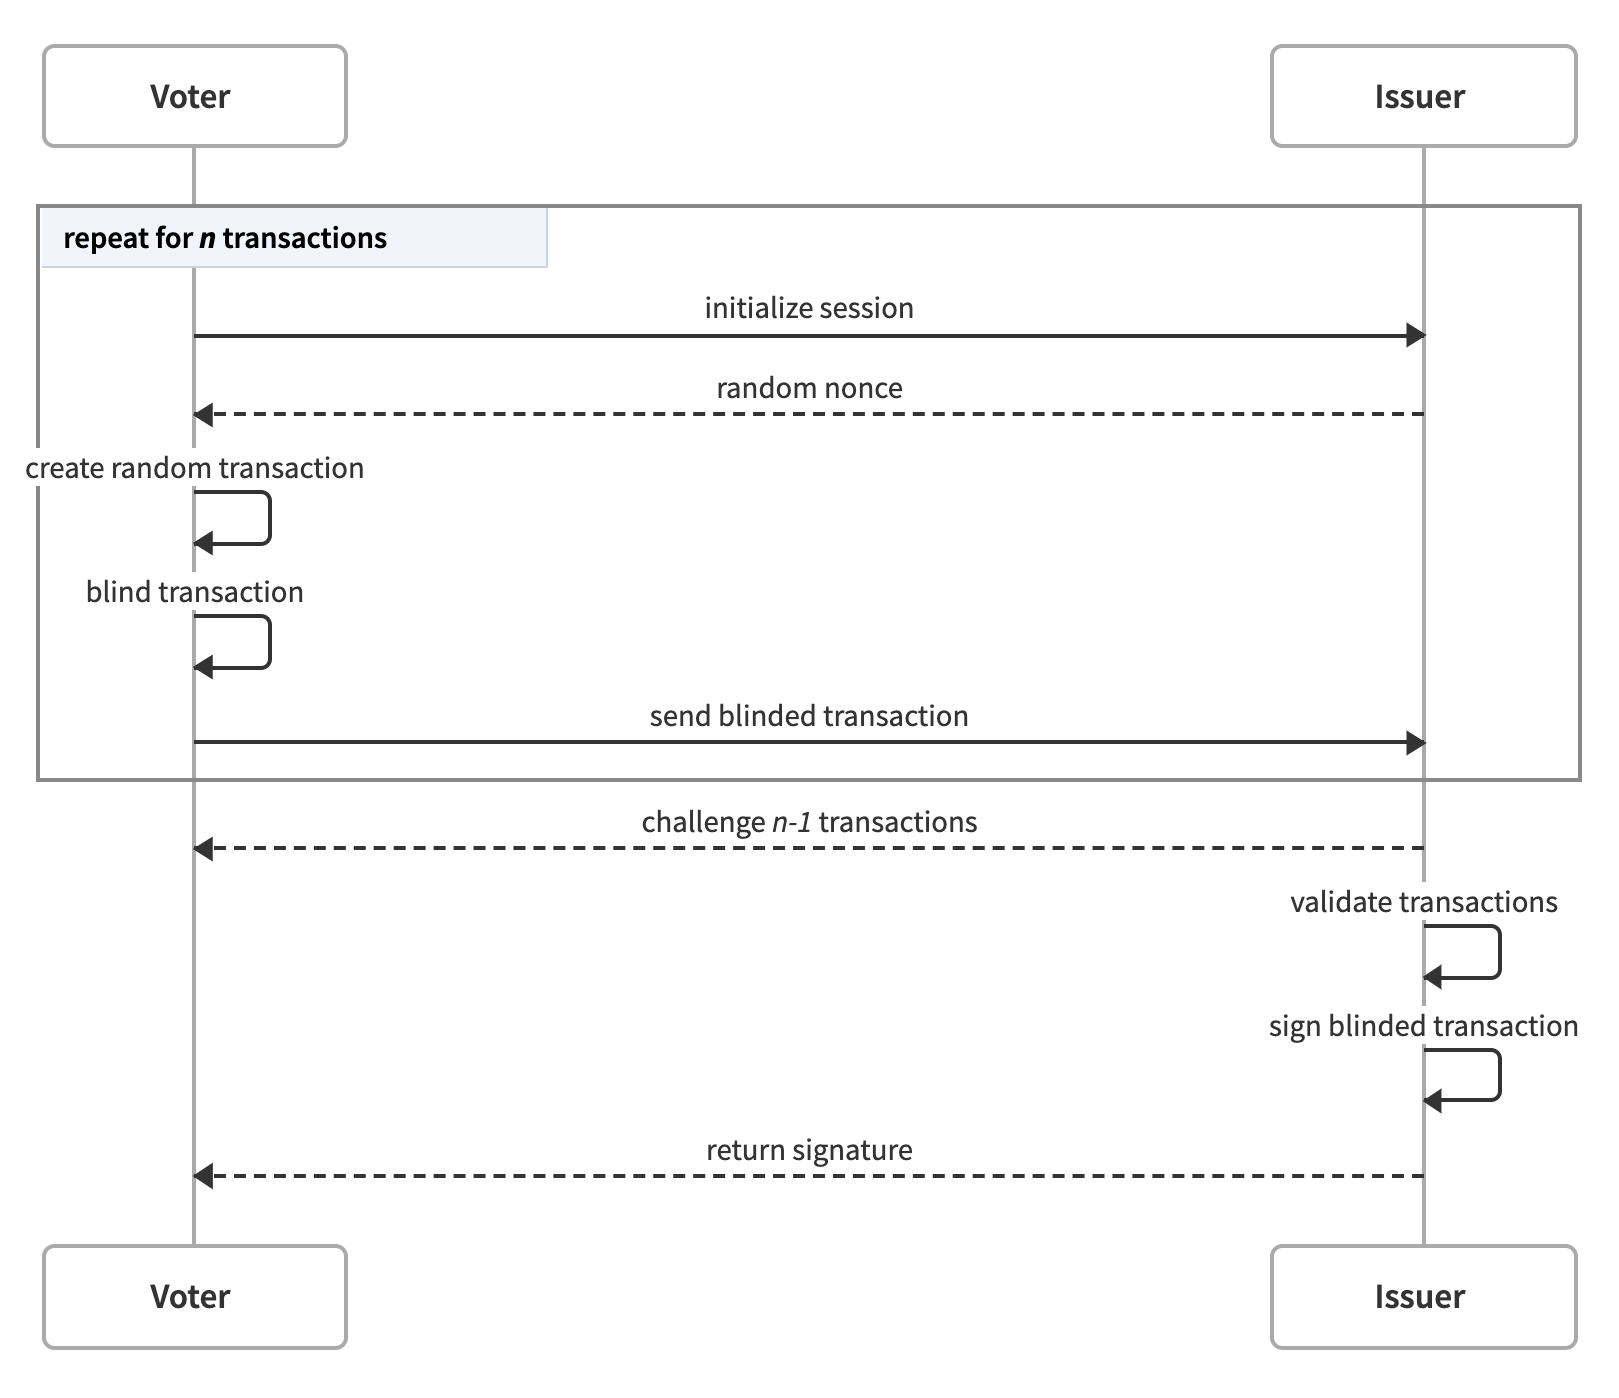
\includegraphics[scale=0.5]{blind-signature.png}

\section{Transaction Fees}
Let’s evaluate the proposed system in the context of transaction fees. To do this we can estimate how much would cost the 2019 Polish parliamentary election, handled by the proposed system. We already know that 18 470 710 people participated in such an election. Each operation on stellar network costs 0.00001XLM. Our vote transaction consists of just one operation (transfer of 1 \textit{vote token}, and so the total cost of transaction also equals 0.00001XLM. We know that the closing price for one Lumen in the day of the election was 0.061 USD. We can easly calculate \(18470710 vote * 0.00001 \frac{XLM}{vote} * 0.061 \frac{USD}{XLM} \approx \textbf{11,27 USD}\). Other operational transactions can be neglected due to very low influence on total sum.

\section{Preparation}
To create such an election, we need an issuer, distribution account, and a new vote token. Creating issuer, distribution account and creating new token is a multi-step process; well described on official stellar documentation. See bootstrap.js for whole flow implementation. Variables that need to be propagated in backend and webpage code are:
• asset name, asset issuer public key, distribution account public key, ballot-box account public key.
• limit of possible vote tokens (number of eligible voters). 
• list of (candidate name, candidate code).
• keypair for encrypting/decrypting transaction MEMO fields before/after election end.

\section{Fully Decentralized Blockchain Application}
In the blockchain world in order to ensure absolute trust, everything should be blockchain contained, which is often hard, impractical and/or expensive. For example one could encode all eligible voter addresses (or better hash of addresses) in smart contract and then allow redeeming vote token only to addresses which are present in there, very similar to traditional election system where all eligible voters are listed on paper. Ballot is issued only if elector is present on such list. While this might work for a small list of addresses, it can become overkill for election when the cost of such a huge smart contract is taken into account. Fortunately, there are already blockchains that allow linking data from outside the blockchain, by using Oracles. To ensure immutability and integrity, such list can be hosted on IPFS (Content Addressed Network) where data is identified by its hash.

\section{System weakness}
In our system, we assumed that Identity Provider and Issuance Server are honest actors. We assumed that we know the total number of eligible voters, and that only eligible voters are able to redeem tokens. The question is how can we know if the authorities doesn't publish greater number of eligible voters and redeem this extra number of tokens to themselves. Being able to significantly influence the election results. Preregistration phase doesn't help here, since malicious government also can take part in it, generating extra tokens. There are some mitigation proposition where it would be required from voter to compute some kind of proof-of-work that would require a lot of computing power by one actor to create a lot of votes.

\section{Results}
The proposed system satisfies all assumed requirements. Each vote is recorded on Blockchain, and everyone can calculate election results without trusting authorities. Thanks to blind signature, Voter can be sure that his decision will be kept private. Unfortunately the system still rely on trust to issuer, who decide who is eligible to receive vote right. If this single point of failure could be eliminated, we would achieve truly decentralized trustless system, without central authorities.
Besides that, we confirmed that blockchain can be used not only for cryptocurrencies, but also in assets tokenization and building dapps (decentralized applications). Stellar is just one of many platforms that could be used in such cases, but it turns out that it handles it very well. What makes Stellar one of the best options in this category is speed and transaction fees. We estimated costs of 2019 Polish parliamentary election to 11,27 USD. To estimate transaction speed we would need to host a local instance of Stellar Horizon API server to isolate from network latency and possible queuing overhead. Doing it would also allow to accurately measure how the proposed system behaves on heavy overload. It would be interesting to compare such system on different blockchain platforms. Source code and demo are available under following links \url{https://github.com/stasbar/stellar-voting}, \url{https://voting.stasbar.com}.

\section{Discussion}
%JS podkreslic zalety systemu, jakie funkcjonalnosci sie udalo zrealizowac, jakie nie jak je mozna skompensowac.

\bibliographystyle{splncs04}
\bibliography{refs}
\end{document}

